
%% bare_conf.tex
%% V1.4b
%% 2015/08/26
%% by Michael Shell
%% See:
%% http://www.michaelshell.org/
%% for current contact information.
%%
%% This is a skeleton file demonstrating the use of IEEEtran.cls
%% (requires IEEEtran.cls version 1.8b or later) with an IEEE
%% conference paper.
%%
%% Support sites:
%% http://www.michaelshell.org/tex/ieeetran/
%% http://www.ctan.org/pkg/ieeetran
%% and
%% http://www.ieee.org/

%%*************************************************************************
%% Legal Notice:
%% This code is offered as-is without any warranty either expressed or
%% implied; without even the implied warranty of MERCHANTABILITY or
%% FITNESS FOR A PARTICULAR PURPOSE! 
%% User assumes all risk.
%% In no event shall the IEEE or any contributor to this code be liable for
%% any damages or losses, including, but not limited to, incidental,
%% consequential, or any other damages, resulting from the use or misuse
%% of any information contained here.
%%
%% All comments are the opinions of their respective authors and are not
%% necessarily endorsed by the IEEE.
%%
%% This work is distributed under the LaTeX Project Public License (LPPL)
%% ( http://www.latex-project.org/ ) version 1.3, and may be freely used,
%% distributed and modified. A copy of the LPPL, version 1.3, is included
%% in the base LaTeX documentation of all distributions of LaTeX released
%% 2003/12/01 or later.
%% Retain all contribution notices and credits.
%% ** Modified files should be clearly indicated as such, including  **
%% ** renaming them and changing author support contact information. **
%%*************************************************************************


% *** Authors should verify (and, if needed, correct) their LaTeX system  ***
% *** with the testflow diagnostic prior to trusting their LaTeX platform ***
% *** with production work. The IEEE's font choices and paper sizes can   ***
% *** trigger bugs that do not appear when using other class files.       ***                          ***
% The testflow support page is at:
% http://www.michaelshell.org/tex/testflow/



\documentclass[conference]{IEEEtran}
% Some Computer Society conferences also require the compsoc mode option,
% but others use the standard conference format.
%
% If IEEEtran.cls has not been installed into the LaTeX system files,
% manually specify the path to it like:
% \documentclass[conference]{../sty/IEEEtran}





% Some very useful LaTeX packages include:
% (uncomment the ones you want to load)


% *** MISC UTILITY PACKAGES ***
%
%\usepackage{ifpdf}
% Heiko Oberdiek's ifpdf.sty is very useful if you need conditional
% compilation based on whether the output is pdf or dvi.
% usage:
% \ifpdf
%   % pdf code
% \else
%   % dvi code
% \fi
% The latest version of ifpdf.sty can be obtained from:
% http://www.ctan.org/pkg/ifpdf
% Also, note that IEEEtran.cls V1.7 and later provides a builtin
% \ifCLASSINFOpdf conditional that works the same way.
% When switching from latex to pdflatex and vice-versa, the compiler may
% have to be run twice to clear warning/error messages.






% *** CITATION PACKAGES ***
%
%\usepackage{cite}
% cite.sty was written by Donald Arseneau
% V1.6 and later of IEEEtran pre-defines the format of the cite.sty package
% \cite{} output to follow that of the IEEE. Loading the cite package will
% result in citation numbers being automatically sorted and properly
% "compressed/ranged". e.g., [1], [9], [2], [7], [5], [6] without using
% cite.sty will become [1], [2], [5]--[7], [9] using cite.sty. cite.sty's
% \cite will automatically add leading space, if needed. Use cite.sty's
% noadjust option (cite.sty V3.8 and later) if you want to turn this off
% such as if a citation ever needs to be enclosed in parenthesis.
% cite.sty is already installed on most LaTeX systems. Be sure and use
% version 5.0 (2009-03-20) and later if using hyperref.sty.
% The latest version can be obtained at:
% http://www.ctan.org/pkg/cite
% The documentation is contained in the cite.sty file itself.






% *** GRAPHICS RELATED PACKAGES ***
%
\ifCLASSINFOpdf
  \usepackage[pdftex]{graphicx}
  % declare the path(s) where your graphic files are
  \graphicspath{{images/}}
  % and their extensions so you won't have to specify these with
  % every instance of \includegraphics
  % \DeclareGraphicsExtensions{.pdf,.jpeg,.png}
\else
  % or other class option (dvipsone, dvipdf, if not using dvips). graphicx
  % will default to the driver specified in the system graphics.cfg if no
  % driver is specified.
  % \usepackage[dvips]{graphicx}
  % declare the path(s) where your graphic files are
  % \graphicspath{{../eps/}}
  % and their extensions so you won't have to specify these with
  % every instance of \includegraphics
  % \DeclareGraphicsExtensions{.eps}
\fi
% graphicx was written by David Carlisle and Sebastian Rahtz. It is
% required if you want graphics, photos, etc. graphicx.sty is already
% installed on most LaTeX systems. The latest version and documentation
% can be obtained at: 
% http://www.ctan.org/pkg/graphicx
% Another good source of documentation is "Using Imported Graphics in
% LaTeX2e" by Keith Reckdahl which can be found at:
% http://www.ctan.org/pkg/epslatex
%
% latex, and pdflatex in dvi mode, support graphics in encapsulated
% postscript (.eps) format. pdflatex in pdf mode supports graphics
% in .pdf, .jpeg, .png and .mps (metapost) formats. Users should ensure
% that all non-photo figures use a vector format (.eps, .pdf, .mps) and
% not a bitmapped formats (.jpeg, .png). The IEEE frowns on bitmapped formats
% which can result in "jaggedy"/blurry rendering of lines and letters as
% well as large increases in file sizes.
%
% You can find documentation about the pdfTeX application at:
% http://www.tug.org/applications/pdftex





% *** MATH PACKAGES ***
%
\usepackage{amsmath}
% A popular package from the American Mathematical Society that provides
% many useful and powerful commands for dealing with mathematics.
%
% Note that the amsmath package sets \interdisplaylinepenalty to 10000
% thus preventing page breaks from occurring within multiline equations. Use:
%\interdisplaylinepenalty=2500
% after loading amsmath to restore such page breaks as IEEEtran.cls normally
% does. amsmath.sty is already installed on most LaTeX systems. The latest
% version and documentation can be obtained at:
% http://www.ctan.org/pkg/amsmath





% *** SPECIALIZED LIST PACKAGES ***
%
%\usepackage{algorithmic}
% algorithmic.sty was written by Peter Williams and Rogerio Brito.
% This package provides an algorithmic environment fo describing algorithms.
% You can use the algorithmic environment in-text or within a figure
% environment to provide for a floating algorithm. Do NOT use the algorithm
% floating environment provided by algorithm.sty (by the same authors) or
% algorithm2e.sty (by Christophe Fiorio) as the IEEE does not use dedicated
% algorithm float types and packages that provide these will not provide
% correct IEEE style captions. The latest version and documentation of
% algorithmic.sty can be obtained at:
% http://www.ctan.org/pkg/algorithms
% Also of interest may be the (relatively newer and more customizable)
% algorithmicx.sty package by Szasz Janos:
% http://www.ctan.org/pkg/algorithmicx




% *** ALIGNMENT PACKAGES ***
%
%\usepackage{array}
% Frank Mittelbach's and David Carlisle's array.sty patches and improves
% the standard LaTeX2e array and tabular environments to provide better
% appearance and additional user controls. As the default LaTeX2e table
% generation code is lacking to the point of almost being broken with
% respect to the quality of the end results, all users are strongly
% advised to use an enhanced (at the very least that provided by array.sty)
% set of table tools. array.sty is already installed on most systems. The
% latest version and documentation can be obtained at:
% http://www.ctan.org/pkg/array


% IEEEtran contains the IEEEeqnarray family of commands that can be used to
% generate multiline equations as well as matrices, tables, etc., of high
% quality.




% *** SUBFIGURE PACKAGES ***
%\ifCLASSOPTIONcompsoc
%  \usepackage[caption=false,font=normalsize,labelfont=sf,textfont=sf]{subfig}
%\else
%  \usepackage[caption=false,font=footnotesize]{subfig}
%\fi
% subfig.sty, written by Steven Douglas Cochran, is the modern replacement
% for subfigure.sty, the latter of which is no longer maintained and is
% incompatible with some LaTeX packages including fixltx2e. However,
% subfig.sty requires and automatically loads Axel Sommerfeldt's caption.sty
% which will override IEEEtran.cls' handling of captions and this will result
% in non-IEEE style figure/table captions. To prevent this problem, be sure
% and invoke subfig.sty's "caption=false" package option (available since
% subfig.sty version 1.3, 2005/06/28) as this is will preserve IEEEtran.cls
% handling of captions.
% Note that the Computer Society format requires a larger sans serif font
% than the serif footnote size font used in traditional IEEE formatting
% and thus the need to invoke different subfig.sty package options depending
% on whether compsoc mode has been enabled.
%
% The latest version and documentation of subfig.sty can be obtained at:
% http://www.ctan.org/pkg/subfig




% *** FLOAT PACKAGES ***
%
%\usepackage{fixltx2e}
% fixltx2e, the successor to the earlier fix2col.sty, was written by
% Frank Mittelbach and David Carlisle. This package corrects a few problems
% in the LaTeX2e kernel, the most notable of which is that in current
% LaTeX2e releases, the ordering of single and double column floats is not
% guaranteed to be preserved. Thus, an unpatched LaTeX2e can allow a
% single column figure to be placed prior to an earlier double column
% figure.
% Be aware that LaTeX2e kernels dated 2015 and later have fixltx2e.sty's
% corrections already built into the system in which case a warning will
% be issued if an attempt is made to load fixltx2e.sty as it is no longer
% needed.
% The latest version and documentation can be found at:
% http://www.ctan.org/pkg/fixltx2e


%\usepackage{stfloats}
% stfloats.sty was written by Sigitas Tolusis. This package gives LaTeX2e
% the ability to do double column floats at the bottom of the page as well
% as the top. (e.g., "\begin{figure*}[!b]" is not normally possible in
% LaTeX2e). It also provides a command:
%\fnbelowfloat
% to enable the placement of footnotes below bottom floats (the standard
% LaTeX2e kernel puts them above bottom floats). This is an invasive package
% which rewrites many portions of the LaTeX2e float routines. It may not work
% with other packages that modify the LaTeX2e float routines. The latest
% version and documentation can be obtained at:
% http://www.ctan.org/pkg/stfloats
% Do not use the stfloats baselinefloat ability as the IEEE does not allow
% \baselineskip to stretch. Authors submitting work to the IEEE should note
% that the IEEE rarely uses double column equations and that authors should try
% to avoid such use. Do not be tempted to use the cuted.sty or midfloat.sty
% packages (also by Sigitas Tolusis) as the IEEE does not format its papers in
% such ways.
% Do not attempt to use stfloats with fixltx2e as they are incompatible.
% Instead, use Morten Hogholm'a dblfloatfix which combines the features
% of both fixltx2e and stfloats:
%
% \usepackage{dblfloatfix}
% The latest version can be found at:
% http://www.ctan.org/pkg/dblfloatfix



% *** PDF, URL AND HYPERLINK PACKAGES ***
%
%\usepackage{url}
% url.sty was written by Donald Arseneau. It provides better support for
% handling and breaking URLs. url.sty is already installed on most LaTeX
% systems. The latest version and documentation can be obtained at:
% http://www.ctan.org/pkg/url
% Basically, \url{my_url_here}.




% *** Do not adjust lengths that control margins, column widths, etc. ***
% *** Do not use packages that alter fonts (such as pslatex).         ***
% There should be no need to do such things with IEEEtran.cls V1.6 and later.
% (Unless specifically asked to do so by the journal or conference you plan
% to submit to, of course. )

\usepackage{multirow}

% correct bad hyphenation here
\hyphenation{op-tical net-works semi-conduc-tor}


\begin{document}
%
% paper title
% Titles are generally capitalized except for words such as a, an, and, as,
% at, but, by, for, in, nor, of, on, or, the, to and up, which are usually
% not capitalized unless they are the first or last word of the title.
% Linebreaks \\ can be used within to get better formatting as desired.
% Do not put math or special symbols in the title.
\title{Predicting Brand Loyalty in Grocery Shoppers}


% author names and affiliations
% use a multiple column layout for up to three different
% affiliations
\author{
\IEEEauthorblockN{Rafael Rivera-Soto}
\IEEEauthorblockA{rivera43@stanford.edu}
\and
\IEEEauthorblockN{Daniel Gardner}
\IEEEauthorblockA{dangard@stanford.edu}
}

% conference papers do not typically use \thanks and this command
% is locked out in conference mode. If really needed, such as for
% the acknowledgment of grants, issue a \IEEEoverridecommandlockouts
% after \documentclass

% for over three affiliations, or if they all won't fit within the width
% of the page, use this alternative format:
% 
%\author{\IEEEauthorblockN{Michael Shell\IEEEauthorrefmark{1},
%Homer Simpson\IEEEauthorrefmark{2},
%James Kirk\IEEEauthorrefmark{3}, 
%Montgomery Scott\IEEEauthorrefmark{3} and
%Eldon Tyrell\IEEEauthorrefmark{4}}
%\IEEEauthorblockA{\IEEEauthorrefmark{1}School of Electrical and Computer Engineering\\
%Georgia Institute of Technology,
%Atlanta, Georgia 30332--0250\\ Email: see http://www.michaelshell.org/contact.html}
%\IEEEauthorblockA{\IEEEauthorrefmark{2}Twentieth Century Fox, Springfield, USA\\
%Email: homer@thesimpsons.com}
%\IEEEauthorblockA{\IEEEauthorrefmark{3}Starfleet Academy, San Francisco, California 96678-2391\\
%Telephone: (800) 555--1212, Fax: (888) 555--1212}
%\IEEEauthorblockA{\IEEEauthorrefmark{4}Tyrell Inc., 123 Replicant Street, Los Angeles, California 90210--4321}}




% use for special paper notices
%\IEEEspecialpapernotice{(Invited Paper)}




% make the title area
\maketitle

% As a general rule, do not put math, special symbols or citations
% in the abstract
\begin{abstract}
The abstract goes here.
\end{abstract}

% no keywords




% For peer review papers, you can put extra information on the cover
% page as needed:
% \ifCLASSOPTIONpeerreview
% \begin{center} \bfseries EDICS Category: 3-BBND \end{center}
% \fi
%
% For peerreview papers, this IEEEtran command inserts a page break and
% creates the second title. It will be ignored for other modes.
\IEEEpeerreviewmaketitle



\section{Introduction}
% no \IEEEPARstart
Brand loyalty is a chief concern for marketers of grocery products. Consumers will often buy the same brand of a household good for their entire lives. It is vital for product marketers to determine which consumers are especially ‘brand loyal’ so that the marketers can target advertising and promotions toward them. 
For most grocery items, consumers are presented with the choice of purchasing a brand name product or a store brand product. Well-known national brands include Kellogg’s cereal, Heinz ketchup, and Tide detergent, while store brands include Costco’s Kirkland, Target’s Market Pantry, and Walmart’s Great Value. Despite a brand product often being more expensive than its store brand counterpart, many consumers prefer the reliability and known quality of the national brand. This brand preference or loyalty widely varies across different households and especially across different product types. We use machine learning techniques to predict a household’s preference for brand name products and determine what factors into that predilection.
For a given product, we label households as ‘brand loyal’ or not based on the brand ratio of their past purchases. Our algorithm takes as inputs the demographics of a household along with product-specific parameters. We then use logistic regression, support vector machines, and adaptive boosting to predict the household’s brand loyalty for that product. We also experiment with using the k-nearest neighbors algorithm to find similar product clusters and utilize these clusters as a feature in our final brand loyalty prediction.

% An example of a floating figure using the graphicx package.
% Note that \label must occur AFTER (or within) \caption.
% For figures, \caption should occur after the \includegraphics.
% Note that IEEEtran v1.7 and later has special internal code that
% is designed to preserve the operation of \label within \caption
% even when the captionsoff option is in effect. However, because
% of issues like this, it may be the safest practice to put all your
% \label just after \caption rather than within \caption{}.
%
% Reminder: the "draftcls" or "draftclsnofoot", not "draft", class
% option should be used if it is desired that the figures are to be
% displayed while in draft mode.
%
%\begin{figure}[!t]
%\centering
%\includegraphics[width=2.5in]{myfigure}
% where an .eps filename suffix will be assumed under latex, 
% and a .pdf suffix will be assumed for pdflatex; or what has been declared
% via \DeclareGraphicsExtensions.
%\caption{Simulation results for the network.}
%\label{fig_sim}
%\end{figure}

% Note that the IEEE typically puts floats only at the top, even when this
% results in a large percentage of a column being occupied by floats.


% An example of a double column floating figure using two subfigures.
% (The subfig.sty package must be loaded for this to work.)
% The subfigure \label commands are set within each subfloat command,
% and the \label for the overall figure must come after \caption.
% \hfil is used as a separator to get equal spacing.
% Watch out that the combined width of all the subfigures on a 
% line do not exceed the text width or a line break will occur.
%
%\begin{figure*}[!t]
%\centering
%\subfloat[Case I]{\includegraphics[width=2.5in]{box}%
%\label{fig_first_case}}
%\hfil
%\subfloat[Case II]{\includegraphics[width=2.5in]{box}%
%\label{fig_second_case}}
%\caption{Simulation results for the network.}
%\label{fig_sim}
%\end{figure*}
%
% Note that often IEEE papers with subfigures do not employ subfigure
% captions (using the optional argument to \subfloat[]), but instead will
% reference/describe all of them (a), (b), etc., within the main caption.
% Be aware that for subfig.sty to generate the (a), (b), etc., subfigure
% labels, the optional argument to \subfloat must be present. If a
% subcaption is not desired, just leave its contents blank,
% e.g., \subfloat[].


% An example of a floating table. Note that, for IEEE style tables, the
% \caption command should come BEFORE the table and, given that table
% captions serve much like titles, are usually capitalized except for words
% such as a, an, and, as, at, but, by, for, in, nor, of, on, or, the, to
% and up, which are usually not capitalized unless they are the first or
% last word of the caption. Table text will default to \footnotesize as
% the IEEE normally uses this smaller font for tables.
% The \label must come after \caption as always.
%
%\begin{table}[!t]
%% increase table row spacing, adjust to taste
%\renewcommand{\arraystretch}{1.3}
% if using array.sty, it might be a good idea to tweak the value of
% \extrarowheight as needed to properly center the text within the cells
%\caption{An Example of a Table}
%\label{table_example}
%\centering
%% Some packages, such as MDW tools, offer better commands for making tables
%% than the plain LaTeX2e tabular which is used here.
%\begin{tabular}{|c||c|}
%\hline
%One & Two\\
%\hline
%Three & Four\\
%\hline
%\end{tabular}
%\end{table}


% Note that the IEEE does not put floats in the very first column
% - or typically anywhere on the first page for that matter. Also,
% in-text middle ("here") positioning is typically not used, but it
% is allowed and encouraged for Computer Society conferences (but
% not Computer Society journals). Most IEEE journals/conferences use
% top floats exclusively. 
% Note that, LaTeX2e, unlike IEEE journals/conferences, places
% footnotes above bottom floats. This can be corrected via the
% \fnbelowfloat command of the stfloats package.


\section{Related Work}
Brand loyalty has been extensively studied by economists and marketing researchers. Often their research focuses on a specific demographic group and observes whether this group has different behavior than the population at large. Bronnenberg et al. examines grocery purchases by consumers who are particularly well-informed about the homogeneity of certain brand and store-brand products and observes that they purchase the cheaper store brand more often than the average shopper. They are able to do this by matching employment information (choosing medical professionals and chefs) with domain-specific products (pain medication and baking goods). In a more recent paper, Bronnenberg et al. examines households that have lived in multiple regions of the United States in their lifetime and finds that the ‘brand capital’ they have developed in the past makes them have different brand loyalties than similar consumers in their current region.


The most common use of machine learning algorithms in consumer behavior research is to create ‘market baskets,’ or products that are frequently purchased together. This is useful when trying to develop marketing campaigns to mesh multiple product categories, but it does little to explain which consumers might prefer to buy a brand of a particular product. As evidence of the increasing interest in applying machine learning to the field, the popular data science website kaggle.com has hosted multiple competitions to develop models related to grocery purchases. These include a problem posed by a marketing research firm to predict when shoppers will visit a store next and how much they will spend, as well as a problem from Walmart to classify different types of shopping trips.


The previous approaches to brand loyalty have studied specific groups and how they behave differently, while machine learning in the grocery space has dealt mostly with clustering of substitute and complementary products. We will instead focus on what characteristics of the average consumer contributes to his or her brand purchasing choices. This analysis allows us to address the most pressing question for marketers - which slice of the population they should focus their limited advertising revenue on to maximize the success of their brand, both in the short term and long term.

\section{Dataset and Features}

\subsection{Dataset}
We use the Nielsen Consumer Panel Dataset from the James M. Kilts Center for Marketing at the University of Chicago Booth School of Business. The Nielsen Company provides scanners to households who keep track of their purchases at grocery stores. This data contains more than three million unique universal product codes (UPCs) from transactions between 2004 and 2014. Households have unique ID numbers and usually remain in the dataset over multiple years. The approximately 60,000 households are located in 50 different major metropolitan areas in the United States, representing a broad spectrum of consumers across the country. For this project we used only the 2014 data, as it contains the most unique UPCs.


The data is stored in four separate datasets: Panelists, which contains all the demographic information about each household; Trips, which contains all shopping trips for all the households; Purchases, which contains all the products purchased and the price paid on all shopping trips; and Products, which connects each UPC with one of 1400 product modules.


Each product module represents a group of UPCs that are essentially substitutes for one another. Examples include CEREAL - READY TO EAT, SEAFOOD-TUNA-SHELF STABLE, DAIRY-MILK-REFRIGERATED, and PAIN REMEDIES - HEADACHE.

\subsection{Preprocessing}
In order to prepare our data to use in our machine learning algorithms, we have to determine the purchase history of each household for a given product, and also calculate certain metrics for that product. An example is helpful for illustration: 

To get household purchase history for product module 5000, we filter the Products dataset for UPCs with product module = 5000. We then merge that UPC file with the Purchases dataset to get a list of all purchases made from product module 5000. We then merge with Trips and then with Panelists and now have a list of all purchases, each labeled with its purchasing household. We then sum the number of purchases each household makes in total and also for the specific brand label = ‘CTL,’ which is the brand code for store brand. We can calculate the number of brand name products they bought by taking \# total purchases - \# ‘CTL’ purchases. The household’s ‘brand loyalty’ is simply \# brand purchases / \# total purchases. 


We also calculate the following metrics for product module 5000: average unit price, average brand/store brand price ratio, and total brand/store-brand purchase ratio. The average unit price is the total \$ spent / \# units purchased. The brand price ratio = (total \$ spent on brand / \# brand units purchased) / (total \$ spent on store brand / \# store brand units purchased). The brand purchase ratio = \# brand purchases / \# total purchases.

We choose a collection of 25 representative products to make predictions about. We require each product to have more than 10,000 purchases in the year and we include a mix of products across departments, from FROZEN FOODS to ALCOHOLIC BEVERAGES to HEALTH \& BEAUTY. We are especially careful to select products that have a variety of household brand loyalty ratios. In general, most households were almost 100% ‘brand loyal’ or not for any given product. It is important to select products that at least have some households that are 100% ‘brand loyal’ and 0% ‘brand loyal’ so that our binary prediction models are meaningful. Some of our selected products are strongly ‘brand’ (detergent), some have mostly off-brand purchases (milk), while others are a mix of both (eggs).

\subsection{Feature Selection}

The demographic information about each household in the Panelists file is quite extensive. It contains the number and age of adults and children, the education and employment information of the male and female head of house, the zip code and residence type, and the household’s race and income. It also contains information about the presence to kitchen appliances, televisions, and internet connection in the home.
	
	
For our machine learning algorithms, we chose as features income, race, household size, age and presence of children, and head male and female education and employment status. Each of these was a categorical variable and required us to create a dummy binary variable for each of its categories. For example, age\textunderscore and\textunderscore presence\textunderscore of\textunderscore children has eight different categories representing combinations of numbers and ages of children in the home. We reduced this to three binary categorical variables: has\textunderscore young\textunderscore children, has\textunderscore children, has\textunderscore teenagers. Age and income did not require dummy variables because their categories were granular and monotonically increasing. One notable feature we omitted was occupation, which simply had too many categories and mostly correlated with income.

\section{Methods}

\subsection{Logistic Regression}
Our initial efforts were concentrated upon whether consumers tend to buy more branded or non-branded products. This is a binary classification task for which we implemented a Logistic Regression model. A Logistic Regression squashes the output of the model in the range $y = \{0,1\} $  using the sigmoid function (Eq. 1). The output values are then interpreted as the probabilities, thus any output greater than 0.5 is classified as belonging to the positive class and to the negative class otherwise (Eq. 2).

\begin{equation}
h_\theta(x) = g(\theta^Tx) =  \frac{1}{1 + e^{-\theta^Tx}}
\end{equation}

\begin{equation}
\begin{aligned}
P(y = 1 | x;\theta) = h_\theta(x) \\
P(y = 0 | x;\theta) = 1 - h_\theta(x)
\end{aligned}
\end{equation}

We based our initial predictions on products whose distributions between branded buyers and non-branded buyers was almost even. We labeled someone as being on the ``branded-buyer" class if they're above the ratio cut-off value of 0.5, all other consumers were labeled as belonging to the``non-branded" class. 

\subsection{Support Vector Machines}
The Support Vector Machine is a discriminative classifier that finds an optimal hyperplane  with the largest margin between the classes. These models also allow us to implicitly map our input features into a high-dimensional feature space where the optimal hyper-plane might result in a better division between the classes. These feature mappings are called kernels. In our implementation, we used the Radial Basis Function (RBF) kernel (Eq. 3). SVM's use a particular choice of the loss function called the ``Hinge Loss" (Eq. 4). To fit this model, we use an algorithm such as Stochastic Gradient Descent to adjusts our weights in such a way that the Hingle Loss is minimized. We used this model in the binary classification model described above and compare the effectiveness.

\begin{equation}
K(x,x') = exp (-\frac{||x-x'||^2}{2\sigma^2})
\end{equation}

\begin{equation}
\delta(z,y) = max \{0,1-yz\}
\end{equation}

\subsection{Boosting}
The idea of this model is to take a weak learning algorithm, that is, any learning algorithm that does slightly better than random and transform it to a strong classifier that does much better than random. Roughly, this method begins by assigning every training example equal weight. It then receives a weak-hypothesis that does well according to the current weights. A weak hypothesis is an algorithm that takes as inputs some distribution (weights) $p$ and outputs a weak learner that does better than random (Eq. 5). After evaluating the results after incorporating the new hypothesis, it re-weights the examples in such a way that incorrect classifications receive higher weights and correct classifications receives lower weights. In this way, boosting is able to create a strong hypothesis that generalizes well to new examples.

\begin{equation}
\sum_{i=1}^{m} p^{(i)} 1 \{y^{(i)} \neq \phi_j(x^{(i)})\}  \leq \frac{1}{2} - \gamma
\end{equation}

\subsection{Softmax Regression}
After our initial efforts, we decided to extend our model to incorporate more than one class. In particular, we chose to divide consumers into three bins using cutoffs at 0.33 and at 0.66. This resulted in the following class division:

\begin{equation}
C=
\begin{cases}
0, \text{if}\ ratio < 0.33 \\
1, \text{if}\ 0.33 \leq ratio < 0.66 \\
2, \text{if}\ ratio \geq 0.66
\end{cases}
\end{equation}

All of our previous models have been binary classifiers. In order to account for more classes we fit a Softmax Regression model. This is a generalization of the Logistic Regression models to multiple classes. In particular, Softmax Regression uses the Multinomial Distribution. The probability that our features take on a certain class is given by Eq. 7.

\begin{equation}
p(y = i | x;\theta) = \frac{e^{\eta_i}}{\sum_{j=1}^{k} e^{\theta_j^Tx}}
\end{equation}

\section{Experiments}

\subsection{Results}

\subsection{Discussion}
Multinomial logistic regression allows us to capture the middle group of brand neutral consumers, so it makes sense that this has the highest accuracy.
The demographic features contributing to brand purchases are somewhat logical. Brands cost more, so higher earners can afford to pay a premium while lower earners opt for off-brand replacements. Older females often make most of a household’s grocery purchases, and they are likely to have settled on a reliable brand. Household size should be explored further, as it is unclear what that indicates about brand loyalty. An interesting discovery is that certain premium products (e.g. brand eggs) are preferred by households with white, educated women. 
Future work could focus on finding a marketing strategy that attracts new customers to a brand. We could predict which groups of consumers will be most likely to switch from off-brand to brand products and then calculate potential profits from these new consumer purchases.

\begin{figure}
\centering
        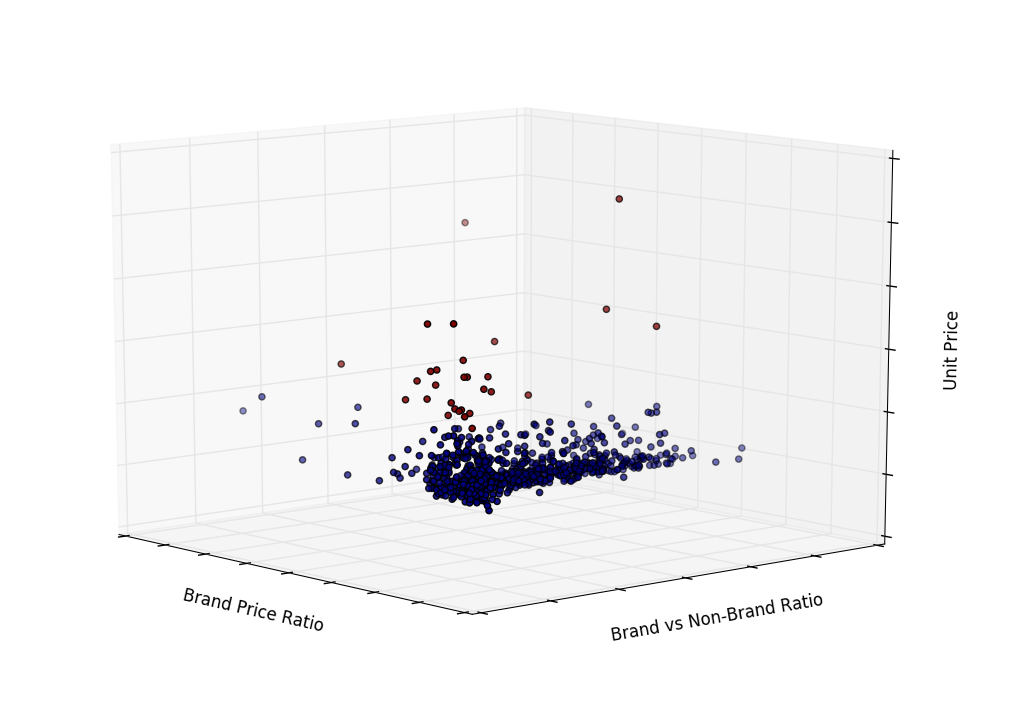
\includegraphics[totalheight=6cm]{clusters}
    \caption{Caption}
    \label{fig:verticalcell}
\end{figure}

\begin{figure}
\centering
        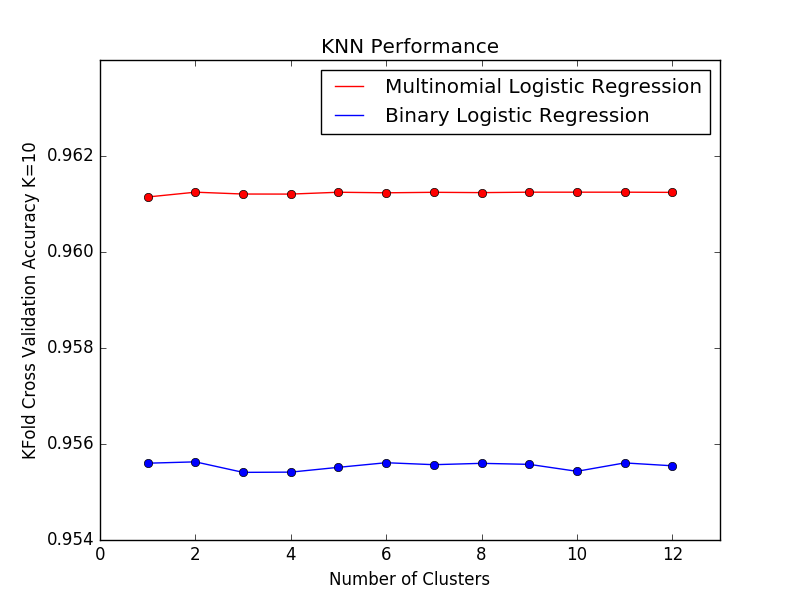
\includegraphics[totalheight=6cm]{cluster-analysis-combined}
    \caption{Caption}
    \label{fig:verticalcell}
\end{figure}

\begin{figure}
\centering
        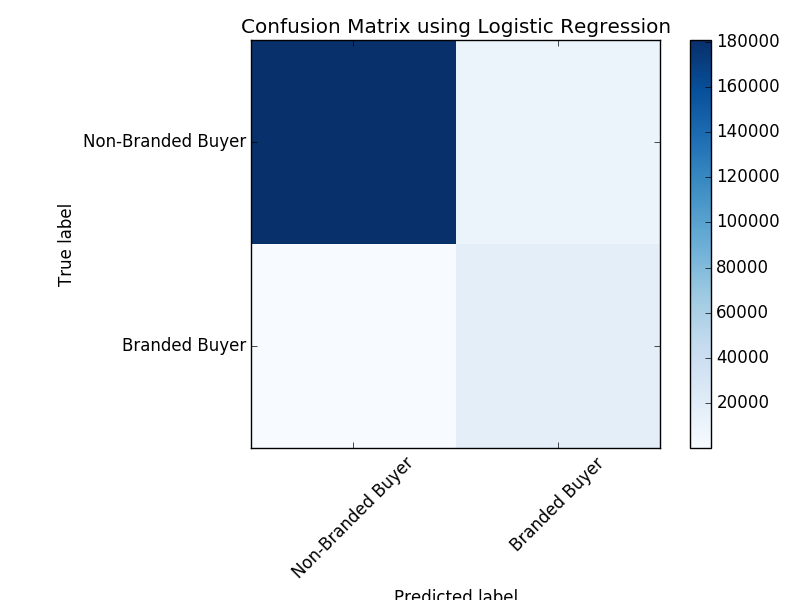
\includegraphics[totalheight=6cm]{confusion-matrix-binary}
    \caption{Caption}
    \label{fig:verticalcell}
\end{figure}

\begin{figure}
\centering
        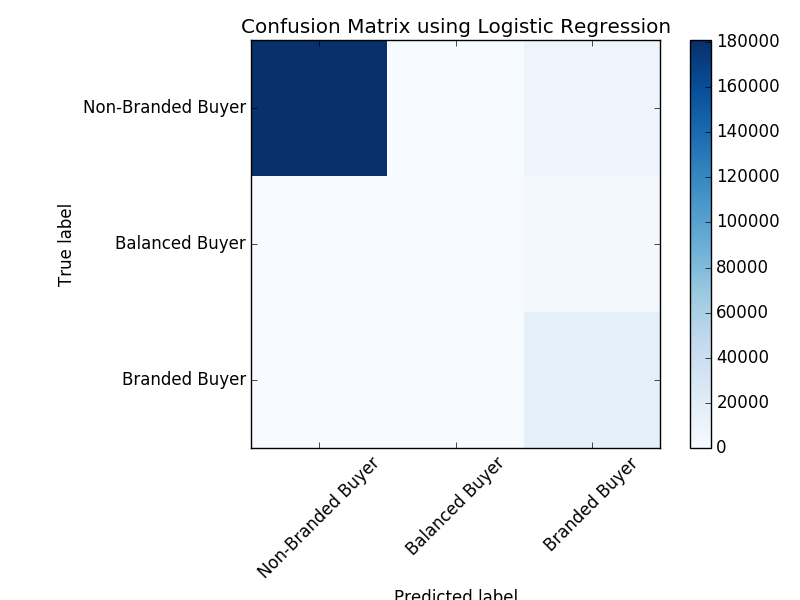
\includegraphics[totalheight=6cm]{confusion-matrix-multinomial}
    \caption{Caption}
    \label{fig:verticalcell}
\end{figure}

\begin{center}
\scalebox{0.5}{
\begin{tabular}{ |c|c|c|c|c|c| } 
\hline
Overall & Eggs & Bacon & Contraceptives & Protein Supplements & Ketchup  \\
\hline
Income & White & Income & Income & Income & Income  \\
Household Size & Female Education & Female Age & Household Size & Household Size & White \\
Female Age & Income & Male Age & Age/Presence of Children & Age/Presence of Children & Female Age \\
\hline
\end{tabular}
}
\end{center}


\section{Conclusion}
The conclusion goes here.




% conference papers do not normally have an appendix


% use section* for acknowledgment


% trigger a \newpage just before the given reference
% number - used to balance the columns on the last page
% adjust value as needed - may need to be readjusted if
% the document is modified later
%\IEEEtriggeratref{8}
% The "triggered" command can be changed if desired:
%\IEEEtriggercmd{\enlargethispage{-5in}}

% references section

% can use a bibliography generated by BibTeX as a .bbl file
% BibTeX documentation can be easily obtained at:
% http://mirror.ctan.org/biblio/bibtex/contrib/doc/
% The IEEEtran BibTeX style support page is at:
% http://www.michaelshell.org/tex/ieeetran/bibtex/
%\bibliographystyle{IEEEtran}
% argument is your BibTeX string definitions and bibliography database(s)
%\bibliography{IEEEabrv,../bib/paper}
%
% <OR> manually copy in the resultant .bbl file
% set second argument of \begin to the number of references
% (used to reserve space for the reference number labels box)
\begin{thebibliography}{1}

\bibitem{IEEEhowto:kopka}
H.~Kopka and P.~W. Daly, \emph{A Guide to \LaTeX}, 3rd~ed.\hskip 1em plus
  0.5em minus 0.4em\relax Harlow, England: Addison-Wesley, 1999.

\end{thebibliography}




% that's all folks
\end{document}


